\documentclass[aspectratio=169]{beamer}
%[handout]

\usetheme[progressbar=frametitle]{metropolis}
\usepackage{appendixnumberbeamer}

\usepackage[utf8]{inputenc}
\usepackage[T1]{fontenc}

\usepackage[brazil]{babel}
\usepackage[outputdir=..]{minted}
\usepackage{xcolor}
\usepackage{soul} % strikethrough
\usepackage{advdate}
\usepackage{graphicx}
\graphicspath{{figs/}}
\usepackage{graphbox}

\usepackage[ampersand]{easylist}

\usepackage{multirow}
\usepackage{multicol}
\usepackage{subcaption}

\usepackage{pgf,tikz}
\usetikzlibrary{shapes,arrows,positioning}
\usetikzlibrary{circuits.logic.US}
\usetikzlibrary{matrix,calc}

\usepackage{karnaugh-map}

\usepackage{pgfpages}
\setbeameroption{hide notes} % Only slides
% \setbeameroption{show only notes} % Only notes
% \setbeameroption{show notes on second screen=right} % Both

% \graphicspath{{../figs/}}

\definecolor{bgc}{rgb}{0.95,0.9,0.95}
\definecolor{links}{HTML}{2A7F7F}
\hypersetup{colorlinks,linkcolor=,urlcolor=links}

\newminted{verilog}{fontsize=\scriptsize, 
    linenos,
    numbersep=8pt,
    bgcolor=bgc,
    tabsize=4,
    framesep=3mm} 
    %frame=lines,

\newcommand{\verilog}[1]{\verilogf{#1}{\footnotesize}}

\newcommand{\verilogf}[2]{\inputminted[fontsize=#2, 
    linenos,
    tabsize=2,
    numbersep=4pt,
    bgcolor=bgc,
    framesep=3mm]{verilog}{../codes/#1.v}
}

\newminted{nasm}{fontsize=\scriptsize, 
		   linenos,
		   numbersep=8pt,
           bgcolor=bgc,
		   framesep=3mm} 

\usepackage{booktabs}
\usepackage[scale=2]{ccicons}

\usepackage{pgfplots}
\usepgfplotslibrary{dateplot}

\usepackage{hyperref}


\usepackage{xspace}
\newcommand{\themename}{\textbf{\textsc{metropolis}}\xspace}



\usepackage{pifont}% http://ctan.org/pkg/pifont
\newcommand{\cmark}{\ding{51}}%
\newcommand{\xmark}{\ding{55}}%

% \tiny	
% \scriptsize
% \footnotesize
% \small	
% \normalsize	
% \large	
% \Large	
% \LARGE	
% \huge	
% \Huge	



\newminted{python}{fontsize=\scriptsize, 
		   linenos,
		   breaklines,
		   numbersep=8pt,
           tabsize=2,
		   framesep=3mm} 
		   
\newminted{verilog}{fontsize=\scriptsize, 
		   linenos,
		   breaklines,
		   numbersep=8pt,
           tabsize=2,
		   framesep=3mm} 
		   




\definecolor{bgc}{rgb}{0.95,0.9,0.95}
\definecolor{links}{HTML}{2A7F7F}
\hypersetup{colorlinks,linkcolor=,urlcolor=links}


% \usepackage[style=apa]{biblatex}
% \addbibresource{mm.bib}


% \author{\large Prof. Ricardo Menotti (\href{mailto:menotti@ufscar.br}{menotti@ufscar.br})}

\newcommand{\newauthor}[2]{
  \parbox{0.50\textwidth}{
    \texorpdfstring
      {
        \centering
        \small #1 \newline
        {\scriptsize{\urlstyle{same}\href{mailto:#2}{#2}\urlstyle{tt}}}
      }
      {#1} \newline
  }
}

\author{
  \newauthor{Prof. Ricardo Menotti}{menotti@ufscar.br}
\and \newauthor{Prof. Luciano de Oliveira Neris}{lneris@ufscar.br}  
%\and \newauthor{Prof. Artino Quintino da Silva Filho}{artino@ufscar.br}
% \and \newauthor{Prof. Maurício Figueiredo}{mauricio@ufscar.br}
% \and \newauthor{Prof. Edilson Kato}{kato@ufscar.br}
% \and \newauthor{Prof. Roberto Inoue}{rsinoue@ufscar.br}
}

\date{Atualizado em: \today}

\institute{\large \textbf{Departamento de Computação} \\
Centro de Ciências Exatas e de Tecnologia \\
Universidade Federal de São Carlos}

\title{Lógica Digital (1001351)}

\titlegraphic{\hfill
\includegraphics[height=1.5cm]{LogoUfscar}}



\subtitle{Mapas de Karnaugh} % 

% https://tex.stackexchange.com/questions/140567/drawing-karnaughs-maps-in-latex
% http://www.texample.net/tikz/examples/karnaugh-diagram/

\begin{document}

\begin{frame}
	\titlepage
\end{frame} 

%%%%%%%%%%%%%%%%%%%%%%%%%%%%%%%%%%%%%%%%%%%%%%%%%%%%%%%%%%%%%%%%%%%%%%%%%%%%%%%%

\section{Estratégias de minimização}

\begin{frame}{\insertsection} % Slide with bullets
	\begin{itemize}
		\item Obter a expressão mínima depende do critério usado;
		\item Exemplo: número de termos na expressão e o número de literais nos termos;
		\begin{itemize}
		    \item Ligeiramente diferente do nosso critério anterior; 
		\end{itemize}
		\item Estratégia intuitiva: encontrar o menor número possível de grupos de 1s que cobrem todos os casos em que a função tem um valor igual a 1;
		\begin{itemize}
		    \item Funciona bem para mapas pequenos, mas precisamos de um método organizado;
		\end{itemize}
    \end{itemize}
\end{frame}

\begin{frame}{\insertsection: terminologia}
    \begin{itemize}
        \item<1-> \textbf{Literal:} cada variável que aparece em um termo de produto, na sua forma normal ou inversa; 
        \item<2-> \textbf{Implicante:} agrupamento de $2^n$ mintermos adjacentes; 
        \begin{itemize}
            \item Ex. $f(x_1,x_2,x_3)=\overline{x}_2$ tem 9 implicantes;
        \end{itemize}
        \item<8-> \textbf{Implicante primo:} implicante que não pode ser alargado;
        \begin{itemize}
            \item Os maiores grupos de 1s que podem ser circulados no mapa;
        \end{itemize}
        \item<9-> \textbf{Implicante primo essencial:} contém pelo menos um mintermo que
não está contido em nenhum outro implicante primo; 
        \item<10-> \textbf{Cobertura:} um conjunto de implicantes que abranja todas as saídas 1 da função; 
        \begin{itemize}
            \item O conjunto de todos os mintermos;
            \item O conjunto de todos os implicantes primos; 
        \end{itemize}
    \end{itemize}
    \vspace{-3cm}
    % \onslide<3>{\centering 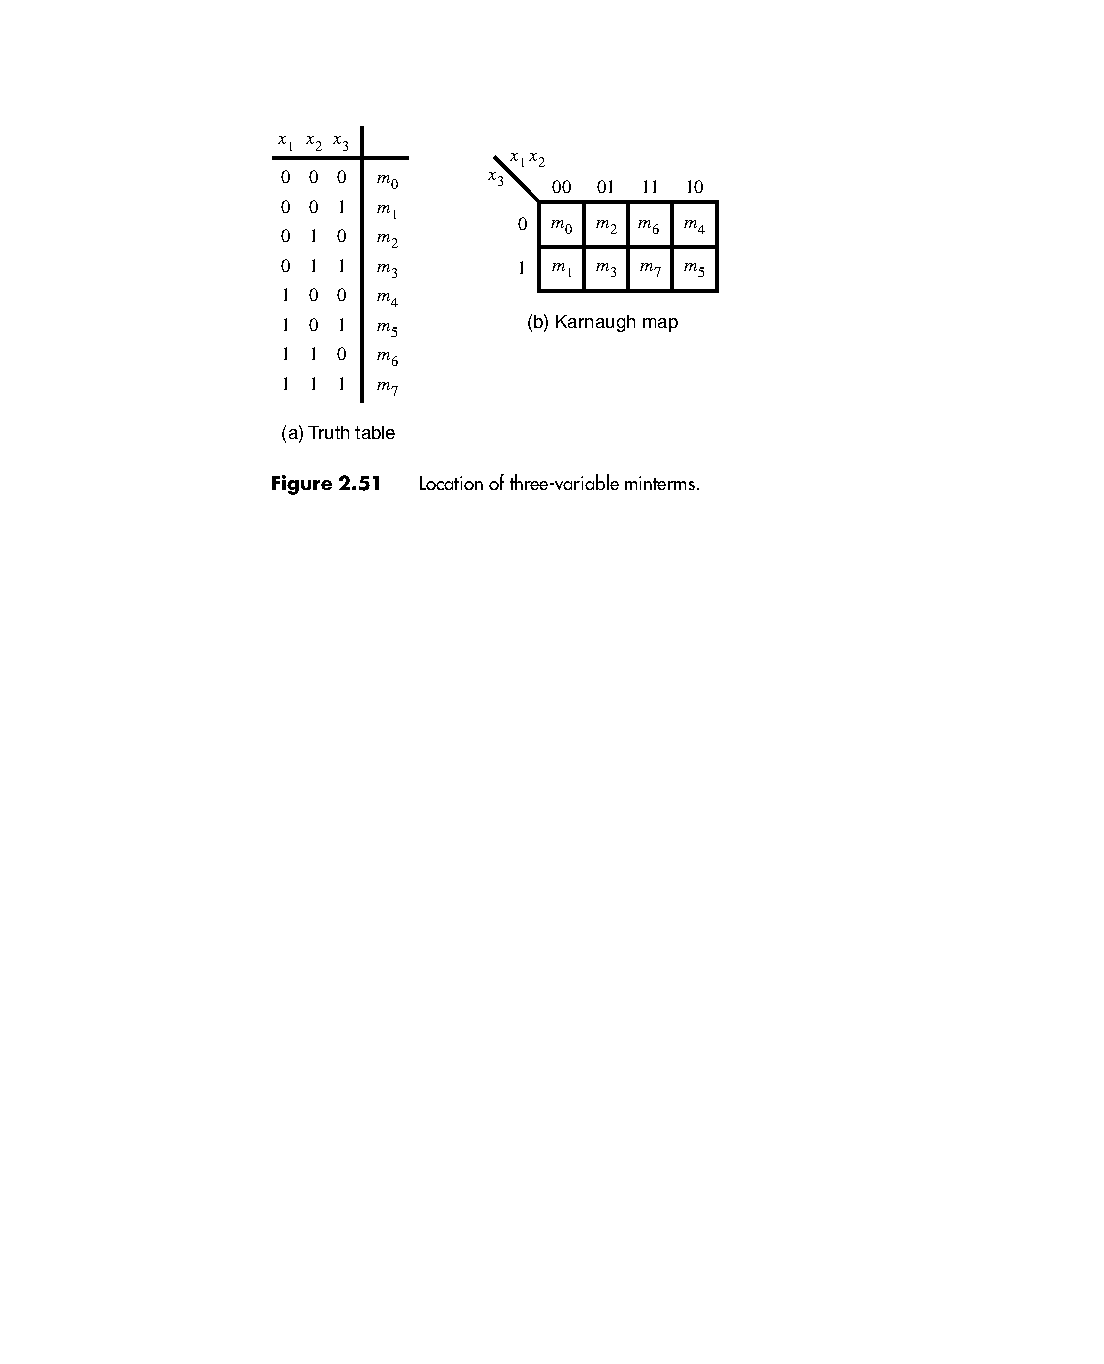
\includegraphics[width=.5\textwidth, trim={3.5cm 3.75cm 0 0}, clip]{VerilogFig2_51}}
    \onslide<3-7>{
    \centering 
    \begin{karnaugh-map}[4][2][1][$x_2x_3$][$x_1$]
    % \manualterms{0,1,2,3,4,5,6,7}
      \minterms{0,1,4,5}
      \maxterms{2,3,6,7}
      \onslide<4-7>{
      \implicant{0}{0}{cyan}
      \implicant{1}{1}{cyan}
      \implicant{4}{4}{cyan}
      \implicant{5}{5}{cyan}}
      \onslide<5-7>{
      \implicant{0}{5`}{green}}
      \onslide<6-7>{
      \implicant{0}{1}{blue}
      \implicant{4}{5}{blue}}
      \onslide<7>{
      \implicant{0}{4}{red}
      \implicant{1}{5}{red}}
    \end{karnaugh-map}}
\end{frame}

\begin{frame}{\insertsection: algoritmo}
    \begin{enumerate}
        \item Gerar todos os implicantes primos para a função;
        \item Encontrar o conjunto dos implicantes primos essenciais;
        \item Se esse oferece cobertura à função, então é a solução desejada; senão, adicionar os implicantes primos \textit{não} essenciais com custo mínimo;
    \end{enumerate}
\end{frame}

\begin{frame}{\insertsection: exemplos}
    \centering
    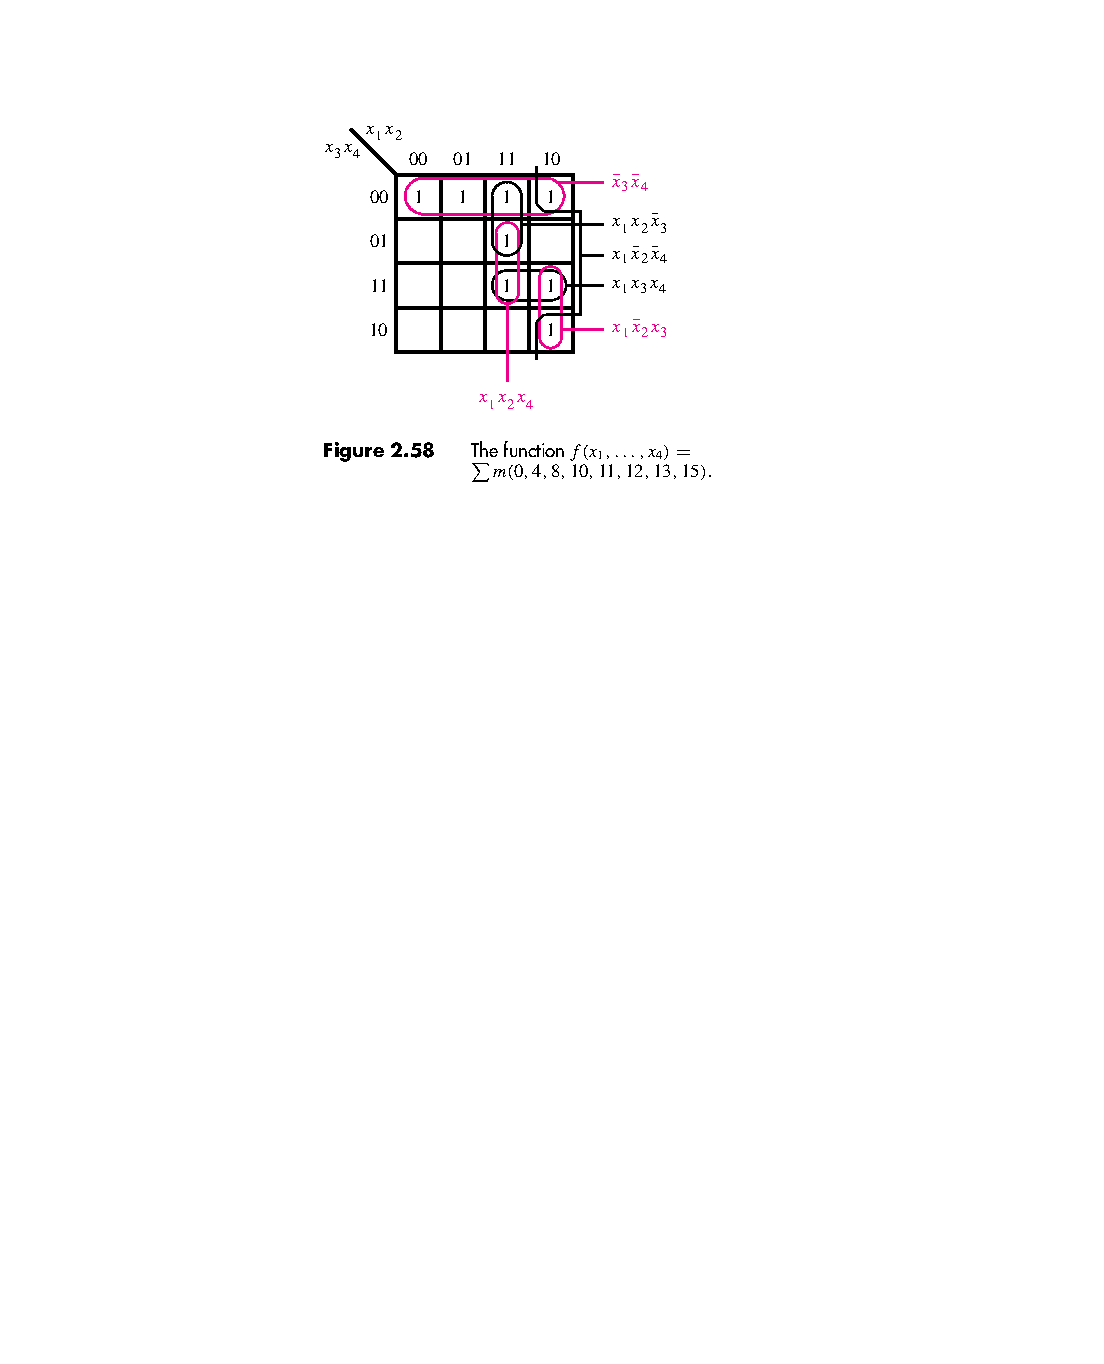
\includegraphics[width=.7\textwidth]{VerilogFig2_58}
\end{frame}

\begin{frame}{\insertsection: exemplos}
    \centering
    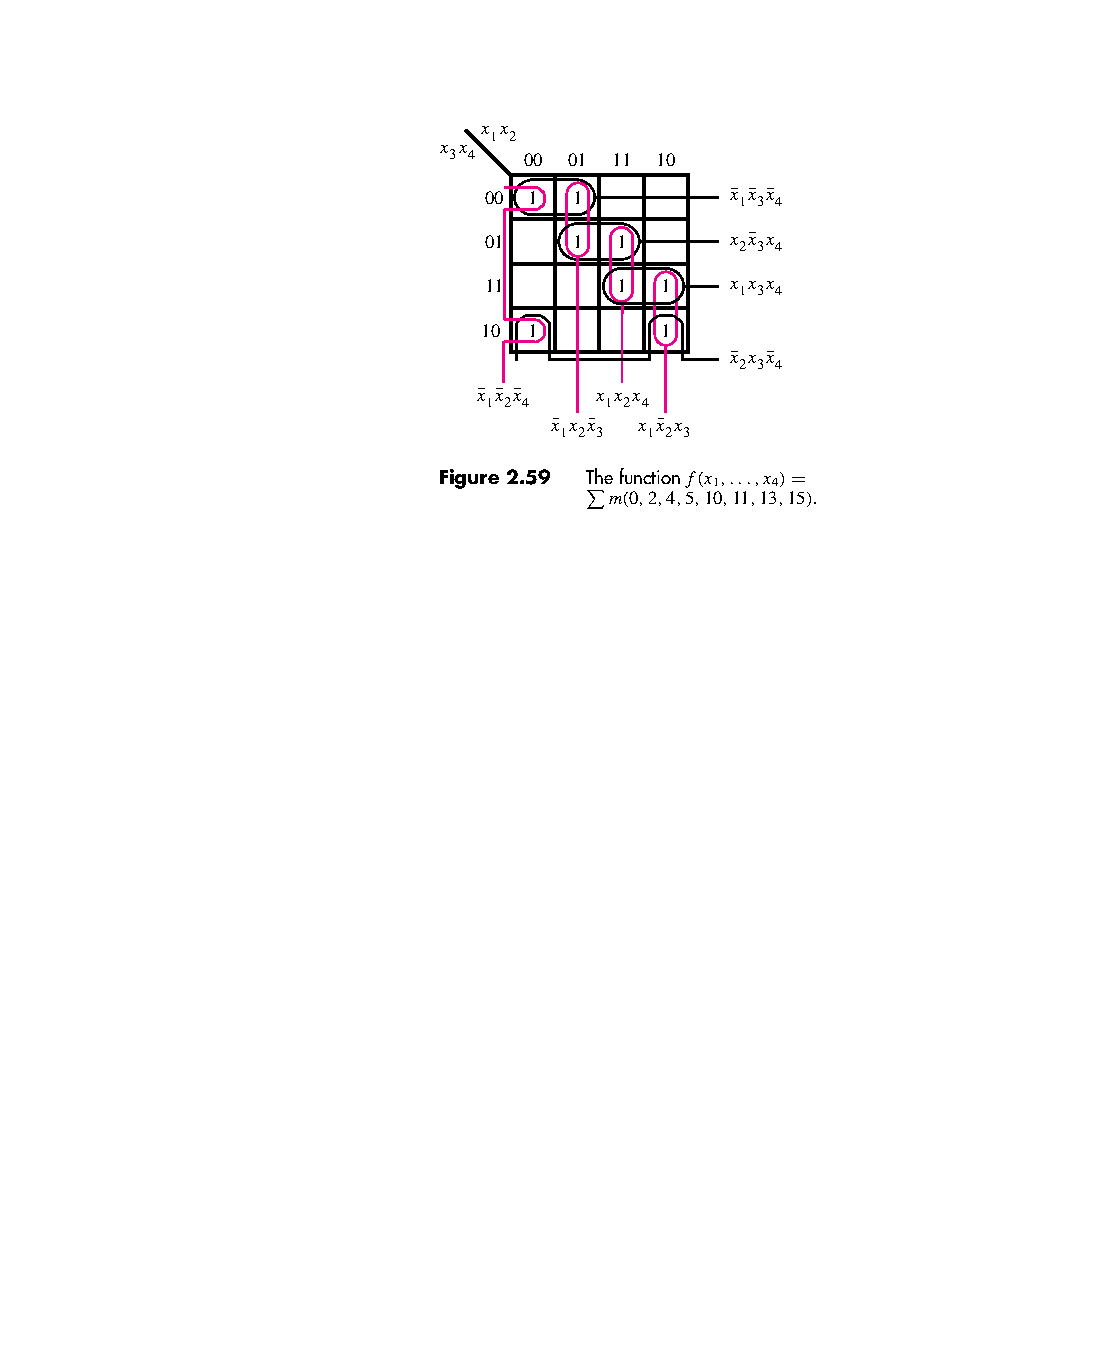
\includegraphics[width=.65\textwidth]{VerilogFig2_59}
\end{frame}

\begin{frame}{\insertsection: exemplos}
    \centering 
    \begin{karnaugh-map}[4][4][1][$x_3x_4$][$x_1x_2$]
    %   \manualterms{0,1,2,3,4,5,6,7,8,9,10,11,12,13,14,15}
      \minterms{1,5,6,7,11,12,13,15}
      \autoterms[0]
       \onslide<2>{
      \implicant{5}{15}
       }
       \onslide<3->{
      \implicant{1}{5}
      \implicant{7}{6}
      \implicant{15}{11}
      \implicant{12}{13}
       }
    \end{karnaugh-map} \\
    $f(x_1, x_2, x_3, x_4) = \Sigma m_{(1,5,6,7,11,12,13,15)}$ \\
    \onslide<4>{$f(x_1, x_2, x_3, x_4) = \overline{x}_1\overline{x}_3x_4 + \overline{x}_1x_2x_3 + x_1x_2\overline{x}_3 + x_1x_3x_4$ }
\end{frame}

\begin{frame}{\insertsection: exemplos}
    \centering 
    \begin{karnaugh-map}[4][4][1][$x_3x_4$][$x_1x_2$]
    %   \manualterms{0,1,2,3,4,5,6,7,8,9,10,11,12,13,14,15}
      \minterms{0,1,5,7,10,14,15}
      \autoterms[0]
      \onslide<2->{
      \implicant{0}{1}
      \implicant{14}{10}
      }
      \onslide<2>{
      \implicant{5}{7}
      \implicant{15}{14}
      \implicant{1}{5}
      \implicant{7}{15}
      }
      \onslide<4>{
      \implicant{5}{7}
      \implicant{15}{14}
      }
      \onslide<5>{
      \implicant{1}{5}
      \implicant{7}{15}
      }
      \onslide<6>{
      \implicant{5}{7}
      \implicant{7}{15}
      }
    \end{karnaugh-map} \\
    $f(x_1, x_2, x_3, x_4) = \Sigma m_{(0,1,5,7,10,14,15)}$ \\
\end{frame}

\section{Bibliografia} %%%%%%%

\begin{frame}{\insertsection} 
	\begin{itemize}
		\item \href{https://www.google.com.br/search?q=filetype\%3Apdf+Fundamentals+of+Digital+Logic+with+Verilog+Design+&oq=filetype\%3Apdf}{Brown, S. \& Vranesic, Z. - Fundamentals of Digital Logic with Verilog Design, 3rd Ed., Mc Graw Hill, 2009}
	\end{itemize}
\end{frame}

\begin{frame}
	\titlepage
\end{frame} 

\end{document}